\documentclass[letterpaper,10pt]{article}

\usepackage{titling}
\usepackage{listings}
\usepackage{url}
\usepackage{setspace}
\usepackage{subfig}
\usepackage{sectsty}
\usepackage{pdfpages}
\usepackage{colortbl}
\usepackage{multirow}
\usepackage{relsize}
\usepackage{amsmath}
\usepackage{fancyvrb}
\usepackage{amsmath,amssymb,amsthm,graphicx,xspace}
\usepackage[titlenotnumbered,noend,noline]{algorithm2e}
\usepackage[compact]{titlesec}
\usepackage[default]{droidserif}
\usepackage[T1]{fontenc}
\usepackage{tikz}
\usetikzlibrary{arrows,automata,shapes,trees,matrix,chains,scopes,positioning,calc}
\tikzstyle{block} = [rectangle, draw, fill=blue!20, 
    text width=2.5em, text centered, rounded corners, minimum height=2em]
\tikzstyle{bw} = [rectangle, draw, fill=blue!20, 
    text width=4em, text centered, rounded corners, minimum height=2em]

\definecolor{namerow}{cmyk}{.40,.40,.40,.40}
\definecolor{namecol}{cmyk}{.40,.40,.40,.40}

\let\LaTeXtitle\title
\renewcommand{\title}[1]{\LaTeXtitle{\textsf{#1}}}


\newcommand{\handout}[5]{
  \noindent
  \begin{center}
  \framebox{
    \vbox{
      \hbox to 5.78in { {\bf ECE155: Engineering Design with Embedded Systems } \hfill #2 }
      \vspace{4mm}
      \hbox to 5.78in { {\Large \hfill #4  \hfill} }
      \vspace{2mm}
      \hbox to 5.78in { {\em #3 \hfill} }
    }
  }
  \end{center}
  \vspace*{4mm}
}

\newcommand{\lecture}[3]{\handout{#1}{#2}{#3}{Lecture #1}}
\newcommand{\tuple}[1]{\ensuremath{\left\langle #1 \right\rangle}\xspace}

\addtolength{\oddsidemargin}{-1.000in}
\addtolength{\evensidemargin}{-0.500in}
\addtolength{\textwidth}{2.0in}
\addtolength{\topmargin}{-1.000in}
\addtolength{\textheight}{1.75in}
\addtolength{\parskip}{\baselineskip}
\setlength{\parindent}{0in}
\renewcommand{\baselinestretch}{1.5}
\newcommand{\term}{Spring 2014}

\singlespace


\begin{document}

\lecture{ 9 --- Version Control}{\term}{Jeff Zarnett \& Patrick Lam}

\section*{Version Control Systems}
We've made you use \emph{version control} for labs,
but just as a dropbox.  In this lecture, we'll talk about some of the
theory of operation behind the use of version control systems.

\begin{itemize}
\item Ever wanted to undo
your changes to software? 
\item Ever needed to collaborate with others to develop software?
\begin{itemize}
\item without
having to email new versions of files to each other and manually integrate
changes?
\end{itemize}
\end{itemize}
Version control lets you do that!

Conceptually, version control stores all of the versions of a set of
files in a \emph{repository}. You can backtrack to any previous
version. You can also investigate previous versions by author, date,
or commit comment. Furthermore, you can merge the changes in your
local copy with some other copy of the set of files, and commit a new
copy, integrating the changes.

\subsection*{Another Trip into the Dark Ages...}

Without version control, if two developers were working on a file, the first one to save his or changes would have them overwritten by the second developer when he or she uploaded the new version to the central server. Here's an example of when Harry was overwritten by Sally:

\begin{center}
	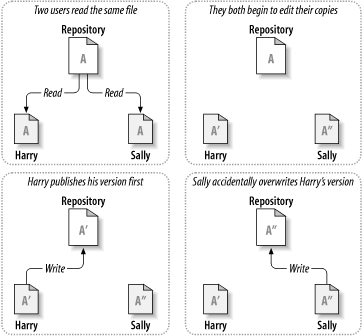
\includegraphics[width=.5\textwidth]{images/ch02dia2.png}
	~\cite{svnbook}
\end{center}

Bugs that were fixed would come back again, new features would break, and so on. There could be a central person whose sole job it is to integrate changes from each developer, but this doesn't scale very well and wastes a lot of human effort. Solution: version control.

\subsection*{Lock-Modify-Unlock}

The first (and now considered almost totally obsolete) attempt at version control used the \emph{lock-modify-unlock} model. The workflow below also explains the name:

\begin{enumerate}
\item To edit a file, you need to \emph{lock} it - you get exclusive access to change the file.
	\item Next, you \emph{modify} the files. You can only modify files you have locked.
	\item Finally, when you are done, you \emph{unlock} the file and it's available for others to lock.
\end{enumerate}

Note that when a file is locked, nobody else can lock it until you unlock it (see step 3), ensuring that there is only one person who has write access to the file at a time (i.e., no concurrent modification). Here's what it looks like when Sally waits for Harry:

\begin{center}
	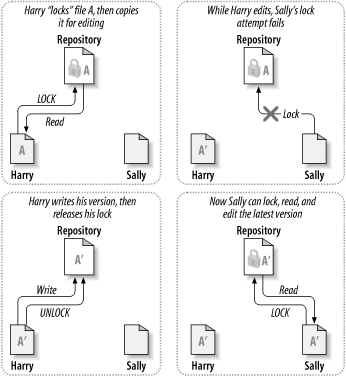
\includegraphics[width=.5\textwidth]{images/ch02dia3.png}
	~\cite{svnbook}
\end{center}

As you can imagine, there are reasons why this model is obsolete. Here are a few of the problems that can occur:

\paragraph{Forgot to Unlock} Locking also requires timely unlocking - if Harry has locked a file, and forgotten to unlock it before he left for vacation, Sally is stuck - she will have to get an administrator to unlock the file for her.

\paragraph{Unnecessary Waiting} Suppose the two developers need to edit the same file but their changes do not overlap. It would be nice if Harry can change the beginning of the file and Sally can change the end, without having to wait for one to finish before the next one starts. With lock-modify-unlock, Sally simply has to wait to make her changes until she can lock the file.

\paragraph{Deadlock} Suppose Harry has \texttt{file1} locked and discovers he needs to also lock \texttt{file2}. He cannot, however, because Sally has \texttt{file2} locked and she wants to get \texttt{file1}. This situation is known as a \emph{deadlock} when it happens in a computer system - and there must be a process for resolving this.

\paragraph{Parallel Modification} if Harry is editing \texttt{file1} and Sally is editing \texttt{file2}. Their changes don't overlap directly, but if the two files interact it's possible that they've made the two files incompatible with one another.

Attempts to address this problem led to:

\subsection*{Copy-Modify-Merge}
Much like its predecessor, the name of the model is best explained as a workflow:

\begin{enumerate}
\item To start working on a project, you check out (\emph{copy}) a
  version of the project, usually the most recent one, to create your
  working copy.
\item Next, you \emph{modify} your copy of the projects, test your
  changes, and commit your changes to the repository.
\item Other developers can then \emph{merge} your changes into their
  working copies, which contain their changes. They will then commit
  their changes as appropriate.
\end{enumerate}
Yes, merging works. Have you tried it?

\begin{center}
	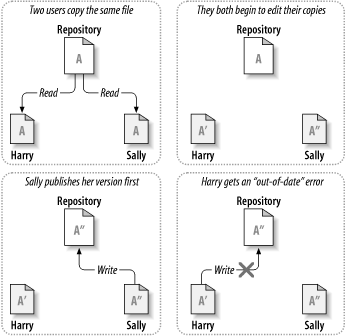
\includegraphics[width=.5\textwidth]{images/ch02dia4.png}
	~\cite{svnbook}
\end{center}

In this situation, Harry and Sally each got a copy of file \texttt{A}. Sally finished her changes first and committed those changes, which updates the repository version of \texttt{A}. Then Harry finishes. But he cannot submit his changes to the repository because the version of \texttt{A} has changed in the meantime. So he needs to perform a merge.

\begin{center}
	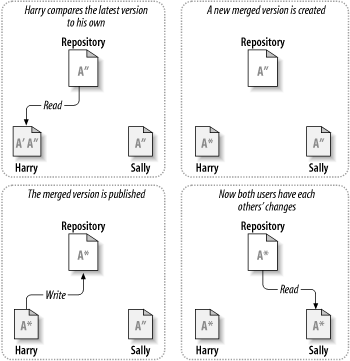
\includegraphics[width=.5\textwidth]{images/ch02dia5.png}
	~\cite{svnbook}
\end{center}

When the merge is performed, the changes from the repository version of \texttt{A} are downloaded and the changes Sally made need to be combined with Harry's changes to produce the newest version of \texttt{A}, shown as \texttt{A''}. Most of the time, the merge will succeed automatically. There is occasionally a \emph{merge conflict}, where the version
control software can't figure out what the right thing should be.  In
that case, you'll have to look at three things: 1) the common
ancestor; 2) your change; and 3) the other change. You can then decide
what the proper result should be. We'll talk more about merge conflicts soon.

Users can work more in parallel (recall from the lecture about multithreading -- less time waiting for others means more time doing useful work). Merge conflicts are usually easy to resolve, and they are infrequent, so less time is spent on locking and unlocking. 

\subsection*{Concurrent Versioning System (CVS)}
One of the very popular solutions for version control is the Concurrent Versioning System \texttt{cvs}. It was developed in the 1980s and at this point the technology is mature and is infrequently updated.

It introduced the concept of \emph{branches}. Revision control sometimes uses the terminology of trees to describe the relationships between different revisions. The main line of the code is called the \emph{trunk}, \emph{main}, or \emph{master}. A parallel line is called a \emph{branch}.

Branches are sometimes merged into their parent (the mainline, usually) which incorporates all of those changes back into the mainline. However, branches may be long-running, such as when Ubuntu creates a release (like 13.04). In this case, changes like bug fixes may be submitted to both the trunk and the branch. This kind of branch will not get merged with the trunk.

Although \texttt{cvs} is still very popular and widely used, but it does have a number of shortcomings:

\paragraph{No Support for Moving or Renaming.} A file that is moved or renamed in \texttt{cvs} is treated as if the old file was deleted and a new file created, so all history information is lost.

\paragraph{Branch Operations are Expensive.} Creating a new branch is expensive and not well supported if the branch is expected to go on for a long time (such as being a supported software release). 

\paragraph{Commits are Not Atomic.} If something goes wrong during a commit, it's possible the repository will be in a corrupted state (with some files changed and others unchanged). If commits are \texttt{atomic}, either the whole commit succeeds or it's cancelled and rolled back to the state before the commit was applied.

Attempts to address the difficulties of \texttt{cvs} led to the creation of SubVersion \texttt{svn}.

\subsection*{Case Study: Subversion}
Subversion is a relatively easy-to-use version control system,
and you've been using it at least to submit source code for the labs.
I'm going to talk about command-line usage; you've been using
{\tt subclipse}.

Here's a useful reference for Subversion: 

Ben Collins-Sussman, Brian W. Fitzpatrick, C. Michael
Pilato. \emph{Version Control with Subversion}.
\url{http://svnbook.red-bean.com/}. Accessed January 27, 2013.

\paragraph{Getting started.} First, you need a copy of a repository.
You can create one from
scratch and then check it out, or you can check out an existing
repository.

To create a repository from scratch, use the {\tt svnadmin} command,
e.g. 

\verb+  svnadmin create c:\svn\repos+

where you've previously created the empty \verb+c:\svn+ directory. Now
you have a repository. Often you won't need to do this, because
someone else will already have created a repository for you. 
You either check out your new repository, or someone else's
repository, before working on it.

To check out a repository, use the {\tt svn checkout} command, 
e.g. 

\verb+  svn checkout http://k9mail.googlecode.com/svn/k9mail/trunk/ k9mail-read-only+

This creates a \emph{working copy}; in this case,
the working copy is in the subdirectory {\tt k9mail-read-only}.

\paragraph{Adding files.} There's an {\tt import} command,
but I don't recommend its use. It is for bringing in a collection of
files that weren't previously version controlled.  Usually, you want
to {\tt svn add} new files, to indicate that they should be in the
repository. A leading cause of build breakage is forgetting to {\tt add}
new files.

\paragraph{Ignoring files.} Tip: editors and compilers always
generate bogus extra files that you don't want to commit, like {\tt
  .obj} files. You can ignore them with
\verb+svn propedit svn:ignore .+, and adding appropriate wildcards
(e.g. {\tt *.obj}) to the ignore list.

\paragraph{Committing files.} Once you're done with your changes,
you need to commit them to the repository. Use the {\tt svn commit}
command to do so. It will prompt you for a commit message, or complain
that it can't get one from you. Good commit messages
are really important~\cite{commit}.

\paragraph{Updating your repository.} You can pull changes from
the repository to your working copy. Use {\tt svn update} to do that.
If all goes well, you'll get output like this:

{
\begin{verbatim}
plam@noether:~/production/11.aosd.modularity$ svn up
D    example.tex
A    studies.tex
U    introduction.tex
A    sketch.tex
U    main.tex
\end{verbatim}
}
The first letter is important. The bad letter is {\tt C}, denoting a
conflict. In that case, you can start by swearing at the fact that you
have to resolve conflicts. Then, you need to go look at the offending
file, which will have conflict markers. The start of the conflict will
have a bunch of \verb+<<<<<<+s, followed by one version of the change,
followed by \verb+======+, and then followed by the conflicting
version. The end-conflict marker is \verb+>>>>>>+.

You resolve the conflict by going into your editor and figuring out
what the file should actually contain. Then you tell svn that you've
resolved the conflict, with {\tt svn resolved}. That allows you to
commit your merged changes.

\paragraph{Stepping back in time.}

Oh no, you committed a bogus change!  You can look at previous
versions by using {\tt svn update} and passing it the {\tt -r}
parameter. This parameter takes a revision number.  Want to know
what's in which revision?  Use {\tt svn log} and read the awesome
commit messages you wrote earlier. Or, you can pass {\tt -r} a date,
e.g. \verb+-r {2011-01-04}+.

Note that {\tt svn update} with a version number just checks out the
version you specified. You can't commit that version. If you want to
merge a previous version with the latest version, use {\tt svn merge}
rather than {\tt svn update}.

\paragraph{Inspecting diffs.} A \emph{diff} shows the difference
between two versions of a file. I recommend reviewing diffs
before committing changes, to avoid embarrassment and to commit
minimal diffs (exclude whitespace). Here is an example of a diff.
{ 
\hspace*{4em} 
\begin{verbatim}
===================================================================
--- Text/abstract.tex	(revision 17379)
+++ Text/abstract.tex	(working copy)
@@ -1,10 +1,10 @@
 Runtime monitoring enables developers to (1) specify important program
 properties and (2) dynamically validate that these properties hold.
 In recent research, we have found that static analysis techniques can,
-in many cases, verify that runtime monitors never trigger.  In
-this paper, we describe a system which enables developers to visualize
-the remaining cases---potential
-points of failure for runtime monitoring properties. Our system
-graphically displays the automata associated with specified runtime
-monitoring properties and enables developers to inspect (and, if
-necessary, fix) the code at each automaton transition.
+in many cases, verify that runtime monitors never trigger.  In this
+paper, we describe a tool which enables developers to visualize the
+remaining cases---potential points of failure for runtime monitoring
+properties. Our tool graphically displays the automata associated with
+specified runtime monitoring properties and enables developers to
+inspect (and, if necessary, fix) the code at each automaton
+transition.
\end{verbatim}
}

Lines with {\tt +} are new, while lines with {\tt -} went away.


\subsection*{Basic workflow}
The basic work cycle of SVN is the following:
\begin{itemize}
\item Update your working copy of the repository using {\tt svn update}.
\item Edit files. Manipulate set of files with {\tt svn add}, {\tt svn delete}, {\tt svn copy}, and {\tt svn move}.
\item Examine changes using {\tt svn status} (to list changed files)
  and {\tt svn diff}.
\item Undo changes, if necessary, using {\tt svn revert}.
\item Commit changes using {\tt svn commit}.
\end{itemize}

\subsection*{svn vs cvs}

SVN was specifically intended to address the shortcomings of cvs, so it does in fact handle many of the things that cvs did not do well.

\paragraph{Atomic commits} If something goes wrong during a commit, it's possible the repository will not be in a corrupted state. Either the entire commit succeeds or the whole thing is rolled back.

\paragraph{Branch Operations.} Branch operations are much less expensive, and there is no longer an expectation that a branch gets merged into the trunk sooner rather than later.

\paragraph{Support for Moving or Renaming.} A file that is moved or renamed in svn is handled better than it was in cvs, but it's still got some issues.

Although it's better in many ways than cvs, there are still issues with svn...

\paragraph{Centralized.} In svn, users all connect to the central repository. If network access is unavailable, none of the source control operations can take place (update, look in the logs, commit, et cetera). 

\paragraph{Slow speed.} It's unfortunately common that both cvs and svn take long enough to do an update of a large amount of source code that it leaves plenty of time for a developer to go get a cup of coffee...

\subsection*{A note on Centralized vs Distributed}
Traditionally, there was one
canonical central repository for a software project.
\emph{Centralized systems} work on that model. So, you copy your
version from the central repository, and commit your changes back to
that repository.

Newer version control systems can be \emph{decentralized}. Every
developer can keep a full copy of the project's history on their
system, and there doesn't need to be a central repository anymore
(although one often exists, in some sense). You can therefore commit
changes to the history on your local computer, without network access.

\subsection*{Git and Mercurial}

One of those decentralized systems is \texttt{git}. It was designed to address some of the shortcomings of other version control systems, but it was also meant to change the way version control is done and not simply be a ``better'' svn. It was created by Linus Torvalds (yes, the Linus Torvalds of the Linux Kernel).

Because git is decentralized, a developer can view the entire history of the repository offline, as well as switch between branches and make commits. Operations are often dramatically faster (because they are done on the local disk and not over the network), and branch operations are not just very inexpensive, but they are the recommended workflow. When you are creating a new feature or fixing a bug, you create a branch, fix your bug in that branch, then merge your branch into the parent. Git also makes it easier to move changes between different branches.

Git still has many concepts that are the same as in svn: adding files, ignoring files, committing files, updating your repository, merging changes, resolving conflicts, and reverting erroneous changes. There are also diffs showing the changes between two versions.

Unfortunately, git is very complex and its learning curve is pretty steep. We'll look at the workflow.

\subsection*{Basic workflow}
The basic work cycle of git is the following:
\begin{itemize}
\item Update your working copy of the repository using {\tt git pull}.
\item Create a feature branch using {\tt git checkout -b}.
\item Edit files. Manipulate set of files with {\tt git add}, {\tt git rm}.
\item Examine changes using {\tt git status} (to list changed files)
  and {\tt git diff}.
\item Undo changes, if necessary, using {\tt git checkout} or {\tt git reset}.
\item Commit changes using {\tt git commit}.
\item Merge your feature branch into the parent branch by first checking the parent branch out ({\tt git checkout}), then doing a {\tt git pull} to update, and then merge with {\tt git merge}.
\item Finally, share your changes with others using {\tt git push}.
\end{itemize}

Finally, a small note on Mercurial (\texttt{hg}). It is also a distributed version control system, similar to git. Although it's easier to learn (it is similar to svn), it doesn't have quite as much out of the box functionality as git. Mercurial is also better supported in Windows. Git and Mercurial are similar enough that there are tools that allow different developers to use their favourite system while accessing the same repository.

\bibliographystyle{alpha}
\bibliography{155}


\end{document}
